\documentclass[aps,pre,superscriptaddress,twocolumn,longbibliography]{revtex4-2}


% Common Package References
\usepackage{graphicx}
\usepackage{dcolumn}
\usepackage{bm}
\usepackage{epstopdf}
\usepackage{algorithm}
\usepackage{algpseudocode}
\usepackage[colorlinks]{hyperref}
\usepackage{amsmath,amsthm,amssymb}
\usepackage{float}
\usepackage{epsfig}
\usepackage{mathrsfs}
\usepackage{multirow}
\usepackage[all]{xy}
\usepackage{pbox}
\usepackage{verbatim}
\usepackage{braket}
\usepackage{mathtools}
\usepackage{tikz}
\usepackage{xcolor}
\usepackage{xfrac}
\usepackage{cleveref}

% Commenting commands

% Template below: replace 'initials' with your initials
%\newcommand{\initials}[1]{{\color{magenta}{\bf [INITIALS: #1]}}}


% Custom Commands
\newcommand{\singlefigure}{0.45\textwidth}


\begin{document}

% TITLE
\title{PRL GitHub Template}

% AUTHORS
\author{John Doe}
\email{john.doe@nottingham.ac.uk}
\affiliation{School of Physics and Astronomy, University of Nottingham, Nottingham, NG7 2RD, UK}
\author{Jane Doe}
\email{jane.doe@nottingham.ac.uk}
\affiliation{School of Physics and Astronomy, University of Nottingham, Nottingham, NG7 2RD, UK}

\date{\today}

\begin{abstract}
This paper outlines the process and intricacies that were explored with creating a drone that is controlled autonomously through reinforcement methods. The method implemented is a state-action value algorithm with a soft policy to ensure all states have a non-zero probability of being taken. This is kept to the bounds of a defined space and set of targets and a specified amount of timesteps. [RESULT] [CONCLUSION] % Loads the abstract.tex file
\end{abstract}

\maketitle

% SECTIONS
% Each section is written in a different file
\section{Introduction}
% Write your introduction here. One can cite\cite{ARXIVEXAMPLE} referenced in the \textit{references.bib} file.
Drones in the current age are becoming more and more popular making the public build their own versions of these drones from their homes. Usually drones are programmed with a flight controller to define how it moves for the task. While there are many ways to control a drone such as user controlled, this project focuses on implementing autonomous flight in which the drone will fly within a defined space to hit a number of targets. The drone that is to be controlled uses two motors which define the thrust independently allowing for navigation within the defined space. The task is to write a flight controller which uses reinforcement learning to have the drone traverse the space to hit as many targets as it can within a specified amount of time.


\section{Results}


Each assessment was done with the following target coordinates.

\begingroup
{\centering
    \begin{tabular}{|l|l|l|l|l|l|}
    \hline
    \textbf{Target} & \textbf{1} & \textbf{2} & \textbf{3} & \textbf{4} & \textbf{5}  \\ \hline
    \textbf{x}      & 0.35       & -0.35      & 0.5        & -0.35      & 0.35        \\ \hline
    \textbf{y}      & 0.3        & 0.4        & -0.4       & 0          & 0.4         \\ \hline
    \end{tabular}
    \begin{tabular}{|l|l|l|l|l|l|}
        \hline
        \textbf{Target} & \textbf{6} & \textbf{7} & \textbf{8} & \textbf{9} & \textbf{10} \\ \hline
        \textbf{x}      & -0.15      & -0.35      & 0.35       & -0.5       & 0.35        \\ \hline
        \textbf{y}      & -0.1       & -0.3       & -0.4       & 0.4        & 0           \\ \hline
        \end{tabular}
}
\endgroup


Each simulation was also run for 3000 simulation steps and 5000 epochs.

In this simulation, the heuristic algorithm hit 5 targets and achieved a value for the sum of rewards as 4894.42, against our chosen reward function.
The following graph shows an example of the Soft state Monti-Carlo state machine algorithm’s results, under the same conditions. \Cref{fig:fig1}.

We modelled the cumulative reward function for any given epoch using the least-squares optimized log function. \Cref{fig:fig1}.

The Logarithmic line for best fit is defined by the following equation:
\begingroup\centering
$1475.01044ln(0.00310817391CumReward) + 1642.65857$
\endgroup

The model has a residual standard deviation of 711.29847146. 
\begin{figure}
    \centering
    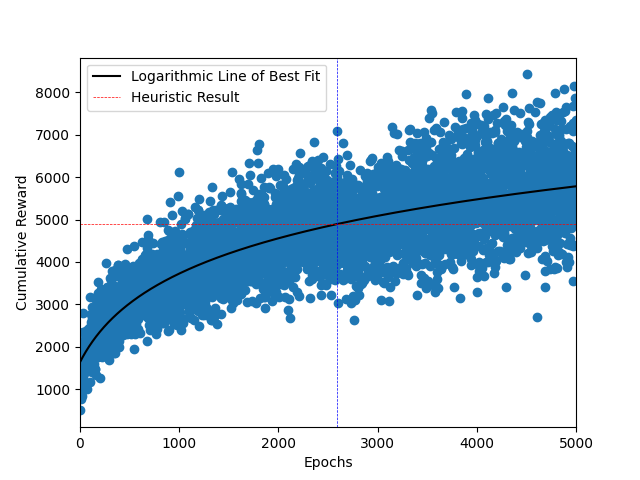
\includegraphics[width=\singlefigure]{figures/figure_2.png}
    \caption{\label{fig:fig1} Shows Logarithmic line of best fit of the data with result of the heuristic.}
\end{figure}

\begin{figure}
    \centering
    \includegraphics[width=\singlefigure]{figures/figure_3.png}
    \caption{\label{fig:fig2} Shows correlation between how many targets hit and cumulative reward for simulation.}
\end{figure}
\section{Conclusions}

The ML alorithm sucessfully demonstrated logarithmic improvement over time.
The cumulative reward function was a successful indicator for the performance of the drone to the high correlation.
The model shows signs of outperforming the Heuristic model but more simulations are required to demonstrate this with statistical significance.
This was a limited of the time contraint of the project.

For future improvements to this work, more simulations are recommended and over more epochs to improve the model.
Through collecting data for different actions and state spaces, it may be possible to improve the performance of the model.


% BIBLIOGRAPHY
\appendix
\bibliography{references}

\end{document}